\section{相对密度}
\label{sec:dens-relative-density}

绝对连续只是一个关于零测集的条件，它没有给出任何函数。本节从相反的方向进入：先给定参考测度和一个非负权重，用积分产生一个新测度，并把权重称为新测度的相对密度，这一方向不需要任何条件。然后问，给定两个测度，能否找到这样的权重。Radon–Nikodym定理回答，在$\sigma$有限的条件下，绝对连续恰好是所需的条件，而且权重在参考测度几乎处处的意义下唯一。

\subsection{由密度生成测度}
\label{sec:dens-weighted-measure}

给定参考测度，怎样用一个权重函数得到新测度？先在有限点集上看清乘数的含义，再用积分把它推广到一般测度，最后说明权重只在几乎处处意义下确定。

\paragraph{有限点集上的质量之比}
设$X=\{a,b,c\}$，目标测度$\nu$给三个点的质量写成向量是$(0.2,0.5,0.3)$。若参考测度是计数测度，每点质量为$1$，从参考质量得到目标质量只需在每点乘以$0.2,0.5,0.3$。若参考测度改为$\mu'=2\delta_a+\delta_b+\delta_c$，点$a$的乘数就要改成$0.2/2=0.1$，另外两点不变。

把乘数写成对角矩阵，这个关系就是矩阵乘向量。对参考$\mu'$，
\[
\begin{pmatrix}0.2\\0.5\\0.3\end{pmatrix}
=\begin{pmatrix}0.1&&\\&0.5&\\&&0.3\end{pmatrix}
\begin{pmatrix}2\\1\\1\end{pmatrix}.
\]
任一子集的目标质量都等于参考质量乘以乘数后求和，例如
\[
\nu(\{a,b\})=0.1\cdot2+0.5\cdot1=0.7 .
\]

图~\ref{fig:dens-mass-ratio}并排画出这两种参考。目标测度在两栏中完全相同，变化的只有参考质量，乘数随之改变。所以乘数描述的是“目标相对于参考”的换算比例，离开参考测度谈乘数没有意义。

\begin{BookInlineFigure}
  \centering
  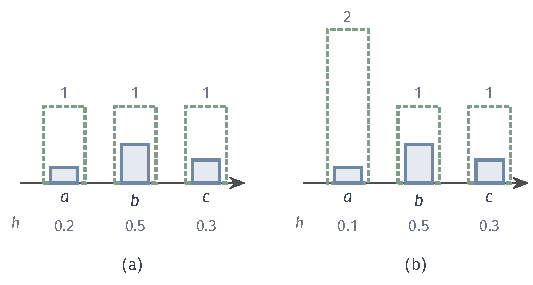
\includegraphics[width=90.255mm]{figures/04-spaces-measures-and-geometry/02-measure/tikz/dens-mass-ratio/figure.pdf}
  \caption{密度是目标质量与参考质量之比。三点集$\{a,b,c\}$上的目标质量$(0.2,0.5,0.3)$（蓝色实心柱）保持不变。(a)参考为计数测度（绿色虚线框高为$1$），每点的密度$h$等于目标质量本身；(b)参考权重改为$(2,1,1)$，点$a$的密度变为$0.2/2=0.1$，其余两点不变。}
  \label{fig:dens-mass-ratio}
\end{BookInlineFigure}

在实轴的长度测度下，每个单点的长度都是$0$，“单点质量相除”变成$0/0$，一般情形不能逐点定义比值，对角矩阵的类比在这里失效。可以保留的是另一半：在每个集合上，参考质量乘以权重再累计，应当得到目标质量。在有限点集上累计是求和，一般情形下就是第~\ref{chap:integration}章的积分。下面约定
\[
\int_Ah\,\mathrm d\mu=\int_Xh\mathbf 1_A\,\mathrm d\mu .
\]

\paragraph{加权测度}
先说明“给定权重，产生测度”总是可行的。这一方向相当于用对角矩阵去乘向量，不需要任何条件。

\begin{theorem}[加权测度]
\label{thm:dens-weighted-measure}
设$(X,\mathcal A,\mu)$是测度空间，$h:X\to[0,+\infty]$可测。令
\begin{equation}
\nu_h(A)=\int_Ah\,\mathrm d\mu ,\qquad A\in\mathcal A .
\label{eq:dens-weighted}
\end{equation}
则$\nu_h$是$(X,\mathcal A)$上的非负测度，并且$\nu_h\ll\mu$。
\end{theorem}

\begin{proof}
空集上的被积函数恒为零，所以$\nu_h(\varnothing)=0$，且$\nu_h$取值于$[0,+\infty]$。

设$A_1,A_2,\ldots\in\mathcal A$两两不交，$A=\bigcup_nA_n$。各$A_n$不交，所以逐点有
\[
h\mathbf 1_A=\sum_{n\geq1}h\mathbf 1_{A_n} .
\]
部分和是递增的非负可测函数列，由单调收敛定理可以逐项积分，得到
\[
\nu_h(A)=\int_Xh\mathbf 1_A\,\mathrm d\mu=\sum_{n=1}^\infty\int_Xh\mathbf 1_{A_n}\,\mathrm d\mu=\sum_{n=1}^\infty\nu_h(A_n).
\]
所以$\nu_h$可数可加。

若$\mu(A)=0$，函数$h\mathbf 1_A$在$\mu$零测集之外为零，其积分为$0$，故$\nu_h(A)=0$，即$\nu_h\ll\mu$。
\end{proof}

证明只用了单调收敛定理，没有要求$\mu$或$h$有限。若$h$在一个正测度集合上取$+\infty$，$\nu_h$可能连$\sigma$有限都不是，但它仍是测度。定理的最后一句说明：凡是能由参考测度加权得到的测度，都相对于参考测度绝对连续。

\begin{definition}[相对密度]
\label{def:dens-relative-density}
设$\mu,\nu$是$(X,\mathcal A)$上的非负测度。若可测函数$h:X\to[0,+\infty]$满足
\begin{equation}
\nu(A)=\int_Ah\,\mathrm d\mu ,\qquad A\in\mathcal A ,
\label{eq:dens-definition}
\end{equation}
就称$h$是$\nu$相对于$\mu$的一个\term{相对密度}（relative density），也称\term{Radon–Nikodym密度}（Radon-Nikodym derivative），记作$\dfrac{\mathrm d\nu}{\mathrm d\mu}=h$；$\mu$称为\term{参考测度}（reference measure）。
\end{definition}

密度的数值同时依赖目标测度与参考测度：上面的三点例子中，同一个$\nu$换一个参考，点$a$的密度就从$0.2$变为$0.1$。记号$\mathrm d\nu/\mathrm d\mu$借用了导数的写法，但它不是对某个坐标求导，而是两种测度之间的换算权重。由定理~\ref{thm:dens-weighted-measure}，密度存在的一个必要条件是$\nu\ll\mu$。

\paragraph{几乎处处版本}
定义说的是“一个”密度。若$h=g$在$\mu$几乎处处成立，则对每个$A$，$h\mathbf 1_A$与$g\mathbf 1_A$也$\mu$几乎处处相等，积分相同，所以$h,g$生成同一个测度。在$[0,1]$上，$h=1$与$g=1+\mathbf 1_{\mathbb Q\cap[0,1]}$都给出$\lambda|_{[0,1]}$，因为二者只在可数集上不同。

因此记号$\mathrm d\nu/\mathrm d\mu$只指其中任一个版本，关于密度的逐点断言，如“$h>0$”“$h<\infty$”，都只在$\mu$几乎处处的意义下才有意义。这与有限点集上不同：在每点都有正质量时，比值逐点确定；在长度下，单点不承载质量，所以单点上的值不算数。

\begin{example}[分段常值密度]
\label{ex:dens-piecewise}
在$[0,1]$上取$\mu=\lambda|_{[0,1]}$，并令
\[
h=\tfrac32\mathbf 1_{[0,1/2)}+\tfrac12\mathbf 1_{[1/2,1]} .
\]
由简单函数的积分，在每一块上把参考质量乘以该块的系数再相加：
\[
\nu_h(E)=\tfrac32\lambda\bigl(E\cap[0,\tfrac12)\bigr)+\tfrac12\lambda\bigl(E\cap[\tfrac12,1]\bigr).
\]
取$E=[0,1]$，得到
\[
\nu_h([0,1])=\tfrac32\cdot\tfrac12+\tfrac12\cdot\tfrac12=\tfrac34+\tfrac14=1 ,
\]
所以$\nu_h$是概率测度。对$E=[1/4,3/4]$，两块的长度各为$\tfrac14$，于是
\[
\nu_h(E)=\tfrac32\cdot\tfrac14+\tfrac12\cdot\tfrac14=\tfrac38+\tfrac18=\tfrac12 .
\]
\end{example}

图~\ref{fig:dens-weighted-measure}(a)中，$E$的质量$\tfrac12$就是$E$上方、密度图像之下的面积。(b)说明在零测点上改动密度不改变面积，这是“几乎处处版本”的几何含义。

\begin{BookInlineFigure}
  \centering
  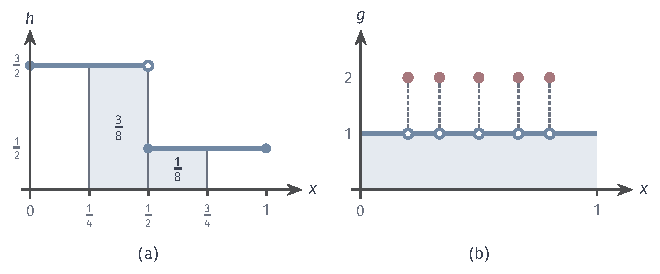
\includegraphics[width=111.693mm]{figures/04-spaces-measures-and-geometry/02-measure/tikz/dens-weighted-measure/figure.pdf}
  \caption{由密度构造测度，以及几乎处处版本。(a)参考测度为$[0,1]$上的长度，密度$h$在$[0,1/2)$上取$3/2$、在$[1/2,1]$上取$1/2$；集合$A=[1/4,3/4]$的质量$\nu_h(A)$是$A$上方的阴影面积$3/8+1/8=1/2$。(b)常数密度$1$与在若干零测点（红点，示意有理点）上改取$2$的函数$g$给出同一测度，因为改动的位置不承载长度。}
  \label{fig:dens-weighted-measure}
\end{BookInlineFigure}

概率论中的概率质量函数与概率密度函数都是这一定义的特例，区别只在参考测度：前者相对于可数集上的计数测度，后者相对于Lebesgue测度，可参考\BookChapterRef{chap:random-variables}{卷七第2章“随机变量的分布”}。一般的密度不要求总积分为一，$\int_Xh\,\mathrm d\mu=\nu(X)$只在目标是概率测度时等于$1$。

概率密度在某点的值也可以大于$1$，上例中$h$在$[0,1/2)$上就等于$\tfrac32$。密度值不是该点的概率，只有在集合上积分后才成为质量。

\subsection{Radon–Nikodym定理}
\label{sec:dens-radon-nikodym}

现在反过来：给定两个测度，能否找到同一个函数$h$，使式~\eqref{eq:dens-definition}对所有可测集同时成立？$\nu\ll\mu$是必要条件。它是否充分是一个真正的问题，因为要同时满足的等式有不可数多个，而绝对连续只告诉我们零测集的信息。

在有限点集上答案是直接的：$\nu\ll\mu$表示$m_i=0$时$p_i=0$，所以在$m_i>0$处令$h_i=p_i/m_i$，在$m_i=0$处任取一个值，就得到密度。一般情形没有逐点比值可用，下面的定理用一种优化的办法把比值“求”出来。

\begin{theorem}[Radon–Nikodym定理]
\label{thm:dens-radon-nikodym}
设$\mu,\nu$是$(X,\mathcal A)$上的$\sigma$有限非负测度，且$\nu\ll\mu$。则存在可测函数$h:X\to[0,+\infty)$，使
\begin{equation}
\nu(A)=\int_Ah\,\mathrm d\mu ,\qquad A\in\mathcal A .
\label{eq:dens-rn}
\end{equation}
若可测函数$g:X\to[0,+\infty]$也满足这一等式，则$g=h$在$\mu$几乎处处成立。
\end{theorem}

把\term{Radon–Nikodym定理}（Radon-Nikodym theorem）与定理~\ref{thm:dens-weighted-measure}对照：那里从$h$得到测度，这里从测度得到$h$。在$\sigma$有限范围内，“$\nu$相对于$\mu$有密度”与“$\nu\ll\mu$”是同一件事。证明先处理两个测度都有限的情形，再用$\sigma$有限性把空间切成可数个有限块。

\paragraph{有限情形：取最大的候选权重}
思路是在所有“处处不超过$\nu$”的权重中找一个积分最大的。把权重想成一层一层往上堆的沙子：每个集合上堆出的量都不能超过$\nu$在该集合上的质量。若某个权重已经堆到不能再高，那么它在每个集合上就应该恰好等于$\nu$。

\begin{lemma}[有限测度的密度存在]
\label{lem:dens-rn-finite}
设$\mu,\nu$是$(X,\mathcal A)$上的有限非负测度，且$\nu\ll\mu$。则存在可测函数$h:X\to[0,+\infty)$，使
\begin{equation}
\nu(A)=\int_Ah\,\mathrm d\mu ,\qquad A\in\mathcal A .
\label{eq:dens-rn-finite}
\end{equation}
\end{lemma}

\begin{proof}
第一步，证明候选权重对取最大值封闭。令
\[
\mathcal G=\Bigl\{g:X\to[0,+\infty]\text{可测}:\ \int_Ag\,\mathrm d\mu\leq\nu(A)\ \ \forall A\in\mathcal A\Bigr\}.
\]
零函数属于$\mathcal G$。设$g_1,g_2\in\mathcal G$，$g=\max(g_1,g_2)$。对任意$A$，令
\[
A_1=A\cap\{g_1\geq g_2\},\qquad A_2=A\cap\{g_1<g_2\}.
\]
二者可测、不交且并为$A$，于是
\[
\begin{aligned}
\int_Ag\,\mathrm d\mu&=\int_{A_1}g_1\,\mathrm d\mu+\int_{A_2}g_2\,\mathrm d\mu\\
&\leq\nu(A_1)+\nu(A_2)=\nu(A),
\end{aligned}
\]
故$g\in\mathcal G$。归纳可知有限个候选的最大值仍是候选。

第二步，用单调序列达到上确界。令
\[
s=\sup_{g\in\mathcal G}\int_Xg\,\mathrm d\mu\leq\nu(X)<\infty .
\]
取$g_n\in\mathcal G$使$\int_Xg_n\,\mathrm d\mu\to s$，再令$h_n=\max(g_1,\ldots,g_n)\in\mathcal G$。$h_n$递增，且
\[
\int_Xg_n\,\mathrm d\mu\leq\int_Xh_n\,\mathrm d\mu\leq s .
\]
令$h=\lim_nh_n$。由单调收敛定理，对每个$A$，
\[
\int_Ah\,\mathrm d\mu=\lim_{n\to\infty}\int_Ah_n\,\mathrm d\mu\leq\nu(A),
\]
所以$h\in\mathcal G$，并且$\int_Xh\,\mathrm d\mu=s$。由于这个积分有限，$h$只在$\mu$零测集上取$+\infty$，把这些值改为$0$不改变任何积分，所以可设$h$处处有限。

第三步，证明剩余质量为零。令
\[
r(A)=\nu(A)-\int_Ah\,\mathrm d\mu\geq0 .
\]
$\nu$与$\nu_h$都是有限测度，逐项相减可知$r$是有限非负测度。又$r\leq\nu$，所以$r\ll\mu$。

反设$r(X)>0$，则由$r\ll\mu$得$\mu(X)>0$。取
\[
\varepsilon=\frac{r(X)}{2\mu(X)} ,\qquad\text{于是}\quad(r-\varepsilon\mu)(X)=\frac{r(X)}2>0 .
\]
$r-\varepsilon\mu$是两个有限测度之差，是有限有符号测度。由第~\ref{chap:measure}章的Hahn分解，存在可测集$P$，使$P$的每个可测子集上$r-\varepsilon\mu\geq0$，$X\setminus P$的每个可测子集上$r-\varepsilon\mu\leq0$。

先说明$\mu(P)>0$。因为$(r-\varepsilon\mu)(X\setminus P)\leq0$，所以
\[
(r-\varepsilon\mu)(P)\geq(r-\varepsilon\mu)(X)>0 ,
\]
从而$r(P)>0$，再由$r\ll\mu$得$\mu(P)>0$。

再说明$h+\varepsilon\mathbf 1_P$仍是候选。对任意$A$，子集$A\cap P$上$r-\varepsilon\mu\geq0$，所以
\[
\varepsilon\mu(A\cap P)\leq r(A\cap P)\leq r(A).
\]
代回候选的积分，得到
\[
\begin{aligned}
\int_A(h+\varepsilon\mathbf 1_P)\,\mathrm d\mu
&=\int_Ah\,\mathrm d\mu+\varepsilon\mu(A\cap P)\\
&\leq\int_Ah\,\mathrm d\mu+r(A)=\nu(A).
\end{aligned}
\]
但它的总积分为$s+\varepsilon\mu(P)>s$，与$s$是上确界矛盾。因此$r(X)=0$，$r$在每个集合上为零，这就是式~\eqref{eq:dens-rn-finite}。
\end{proof}

第三步说明了为什么最大候选不留剩余：只要剩余质量$r$不为零，Hahn分解就能找到一块正测度区域，在那里$r$至少是参考测度的$\varepsilon$倍，于是可以把权重再加高$\varepsilon$。下面用一个两点的例子，把这一步的每个数都算出来。

\begin{example}[剩余质量怎样把候选抬高]
\label{ex:dens-rn-step}
取$X=\{a,b\}$，$\mu=\delta_a+2\delta_b$，$\nu=3\delta_a+\delta_b$。候选权重$g$只有两个数$g_a,g_b$，它在单点上的条件是
\[
g_a\cdot1\leq3,\qquad g_b\cdot2\leq1 .
\]
于是积分最大的候选是$(3,\tfrac12)$，它恰好就是质量之比，并且$s=3+1=4=\nu(X)$。

假设手里的候选还没到最大，取$h=(2,\tfrac12)$，它的总积分是$2+1=3<4$。剩余质量是
\[
r=\nu-h\mu=(3,1)-(2,1)=(1,0),\qquad r(X)=1 .
\]
证明中的$\varepsilon$取为
\[
\varepsilon=\frac{r(X)}{2\mu(X)}=\frac1{2\cdot3}=\frac16 .
\]
于是$r-\varepsilon\mu$在两点的值为
\[
1-\tfrac16\cdot1=\tfrac56,\qquad0-\tfrac16\cdot2=-\tfrac13 ,
\]
两数相加正好是$r(X)/2=\tfrac12$。Hahn分解的正集是$P=\{a\}$。

把$h$在$P$上加高$\varepsilon$，得到$h'=(\tfrac{13}6,\tfrac12)$。它在两点产生的质量是
\[
\tfrac{13}6\cdot1=\tfrac{13}6\leq3,\qquad\tfrac12\cdot2=1\leq1 ,
\]
仍是候选，而总积分从$3$升到$\tfrac{13}6+1=\tfrac{19}6$。只要$r$不为零，这样的抬高总能进行，所以最大的候选不留剩余。
\end{example}

图~\ref{fig:dens-rn-candidate}用连续的例子示意同一步。图中的$f$在证明中事先未知，这里画出只为便于观察；重要的是绿色条带仍在$f$之下，所以抬高后的函数仍是候选。

\begin{BookInlineFigure}
  \centering
  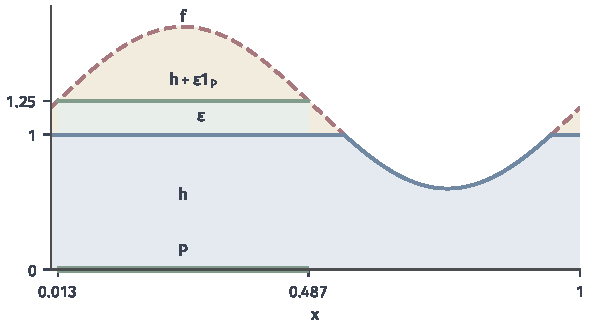
\includegraphics[width=100mm]{figures/04-spaces-measures-and-geometry/02-measure/matplotlib/dens-rn-candidate/figure.pdf}
  \caption{有限情形证明第三步的示意。参考测度为$[0,1]$上的长度，目标测度的密度$f(x)=1.2+0.6\sin(2\pi x)$（红色虚线）。候选$h=\min(f,1)$（蓝色实线）之下的质量已被表示，$h$与$f$之间的黄色区域是剩余质量$r$。取$\varepsilon=0.25$，正集$P=\{f-h\geq\varepsilon\}$约为$[0.013,0.487]$；在$P$上加高$\varepsilon$的绿色条带仍在$f$之下，所以$h+\varepsilon\mathbf 1_P$仍是候选而总积分更大。}
  \label{fig:dens-rn-candidate}
\end{BookInlineFigure}

\begin{proof}[定理~\ref{thm:dens-radon-nikodym}的证明]
先作有限分块。由$\sigma$有限性，存在两两不交的可测集$A_i$覆盖$X$且$\mu(A_i)<\infty$，以及两两不交的可测集$B_j$覆盖$X$且$\nu(B_j)<\infty$。可数族$\{A_i\cap B_j\}$两两不交、覆盖$X$，每块上$\mu,\nu$都有限，把它们排成一列$X_1,X_2,\ldots$。

再证存在性。对每个$k$，令
\[
\mu_k(A)=\mu(A\cap X_k),\qquad\nu_k(A)=\nu(A\cap X_k).
\]
这是两个有限测度，且$\nu_k\ll\mu_k$。由引理~\ref{lem:dens-rn-finite}，存在有限值可测函数$h_k$，使
\[
\nu(A\cap X_k)=\int_Ah_k\,\mathrm d\mu_k=\int_Ah_k\mathbf 1_{X_k}\,\mathrm d\mu ,
\]
后一个等号先对指示函数核对，再经简单函数与单调收敛推广。

令$h=\sum_kh_k\mathbf 1_{X_k}$，各$X_k$不交，每点至多一项非零，$h$有限且可测。由$\nu$的可数可加性与非负级数的逐项积分，
\[
\nu(A)=\sum_k\nu(A\cap X_k)=\sum_k\int_Ah_k\mathbf 1_{X_k}\,\mathrm d\mu=\int_Ah\,\mathrm d\mu .
\]

最后证唯一性。设$g:X\to[0,+\infty]$也满足等式。固定$k$，令$D=X_k\cap\{h>g\}$，则
\[
\int_Dh\,\mathrm d\mu=\nu(D)=\int_Dg\,\mathrm d\mu ,
\]
两边不超过$\nu(X_k)<\infty$，于是$\int_D(h-g)\,\mathrm d\mu=0$。被积函数在$D$上严格为正，所以$\mu(D)=0$。同理$\mu(X_k\cap\{g>h\})=0$。对$k$取可数并，$\{g\neq h\}$是$\mu$零测集。
\end{proof}

唯一性证明中只有一处用到有限性：$\nu(X_k)<\infty$才能把两个相等的积分相减。这里实际只需要$\nu$是$\sigma$有限的。缺少这一条件时唯一性可以失败：单点空间$X=\{0\}$上取$\mu(\{0\})=+\infty$，$\nu=\mu$，常数$1$与常数$2$都满足
\[
\int_{\{0\}}h\,\mathrm d\mu=+\infty=\nu(\{0\}),
\]
却在一个$\mu$测度为$+\infty$的集合上不同。所以密度只在$\mu$几乎处处的意义下唯一，而且这一唯一性依赖目标测度的$\sigma$有限性。

\paragraph{有限性条件不能随意去掉}
存在性同样依赖参考测度的$\sigma$有限性。在$[0,1]$的Borel集上取计数测度$c$与Lebesgue测度$\lambda$。$c(A)=0$只在$A=\varnothing$时成立，所以$\lambda\ll c$。若存在可测$h\geq0$使$\lambda(A)=\int_Ah\,\mathrm dc$，取$A=\{x\}$，就得到
\[
0=\lambda(\{x\})=h(x)c(\{x\})=h(x).
\]
于是$h$处处为零，却要给出$\lambda([0,1])=1$，矛盾。失效的原因在于$c$的有限测度集只能是有限集，可数个有限集之并盖不住$[0,1]$，$c$不是$\sigma$有限的。

这个反例说明定理不能无条件推广，但不说明$\sigma$有限是密度存在的必要条件。仍以$c$为参考，$\delta_0$有密度$\mathbf 1_{\{0\}}$，因为
\[
\int_A\mathbf 1_{\{0\}}\,\mathrm dc=c(A\cap\{0\})=\delta_0(A).
\]
$\sigma$有限是本章采用的一组充分条件。

\paragraph{有限有符号测度的密度}
第~\ref{chap:measure}章的有限有符号测度允许集合质量为负，它由Jordan分解写成两个有限测度之差$\eta=\eta^+-\eta^-$，总变差为$\lvert\eta\rvert=\eta^++\eta^-$。不能把上面的定理直接套到任意两个测度之差上：两个无限测度之差可能在某些集合上是$\infty-\infty$，根本没有定义。对有限有符号测度，可以对两个变差分别求密度。

\begin{theorem}[有限有符号测度的密度]
\label{thm:dens-signed}
设$\mu$是$(X,\mathcal A)$上的$\sigma$有限非负测度，$\eta$是有限有符号测度。则$\lvert\eta\rvert\ll\mu$当且仅当存在$\mu$可积的实值函数$h$，使
\begin{equation}
\eta(A)=\int_Ah\,\mathrm d\mu ,\qquad A\in\mathcal A .
\label{eq:dens-signed}
\end{equation}
此时$h$在$\mu$几乎处处意义下唯一，并且对每个$A\in\mathcal A$，
\begin{equation}
\eta^\pm(A)=\int_Ah^\pm\,\mathrm d\mu,\qquad\lvert\eta\rvert(A)=\int_A\lvert h\rvert\,\mathrm d\mu ,
\label{eq:dens-signed-parts}
\end{equation}
其中$h^+=\max(h,0)$，$h^-=\max(-h,0)$。
\end{theorem}

\begin{proof}
设$\lvert\eta\rvert\ll\mu$。由$\eta^\pm\leq\lvert\eta\rvert$得$\eta^\pm\ll\mu$。$\eta^\pm$是有限测度，由定理~\ref{thm:dens-radon-nikodym}得到有限值密度$h_1,h_2$，并且
\[
\int_Xh_1\,\mathrm d\mu=\eta^+(X)<\infty,\qquad\int_Xh_2\,\mathrm d\mu=\eta^-(X)<\infty ,
\]
二者都可积。令$h=h_1-h_2$，由可积函数积分的线性性，$h$满足式~\eqref{eq:dens-signed}。

反过来，设式~\eqref{eq:dens-signed}成立且$h$可积。令$P=\{h\geq0\}$。$P$的每个可测子集上$\eta\geq0$，补集的每个可测子集上$\eta\leq0$，所以$P$与$X\setminus P$构成$\eta$的一组Hahn分解。由Jordan分解，
\[
\eta^+(A)=\eta(A\cap P)=\int_Ah^+\,\mathrm d\mu ,
\]
\[
\eta^-(A)=-\eta(A\setminus P)=\int_Ah^-\,\mathrm d\mu .
\]
两式相加就得到$\lvert\eta\rvert$的表示，这就是式~\eqref{eq:dens-signed-parts}。由定理~\ref{thm:dens-weighted-measure}，$\lvert\eta\rvert\ll\mu$。

这一段对前一段构造的$h$同样适用，所以式~\eqref{eq:dens-signed-parts}在两个方向上都成立。

唯一性方面，若可积的$h,h'$都满足式~\eqref{eq:dens-signed}，令$D=\{h>h'\}$，则两个有限积分相等，得到
\[
\int_D(h-h')\,\mathrm d\mu=0 .
\]
被积函数在$D$上严格为正，所以$\mu(D)=0$。交换$h,h'$得$\mu(\{h'>h\})=0$，于是$h=h'$在$\mu$几乎处处成立。
\end{proof}

定理把集合层面的正负分解翻译成函数层面的正负部：Hahn分解的正区域可以取为$\{h\geq0\}$，Jordan分解的两项就是$h^+$与$h^-$分别生成的测度。可积性在这里是自然的，因为由式~\eqref{eq:dens-signed-parts}，$\lvert h\rvert$的积分就是有限的总变差$\lvert\eta\rvert(X)$。

例如$[0,1]$上$h(x)=1-2x$生成的$\eta$，正集是$P=[0,\tfrac12]$，两个变差的总质量都可以算出：
\[
\eta^+([0,1])=\int_0^{1/2}(1-2x)\,\mathrm dx=\tfrac14,\qquad\eta^-([0,1])=\int_{1/2}^1(2x-1)\,\mathrm dx=\tfrac14 .
\]
所以$\eta([0,1])=0$，正负质量完全抵消，而$\lvert\eta\rvert([0,1])=\tfrac12$记录了被抵消掉的变化总量。
